\begin{frame}{}
    \begin{center}
        \LARGE Backup
    \end{center}
\end{frame}
    


\begin{frame}{Estrategia de Simulacion}
El elemento iniciador se encuentra en la función \texttt{genera\_v5.py} versión 5, con este se incluye una descripción de opciones que hacen que sea adaptable ante situaciones alternativas a su configuración original:\\
\begin{scriptsize}
\texttt{
\begin{tabular}{ll}
genera\_v5.py [-h] & [-Event EVENT] [-MNeuD MNEUD] [-MNeuD MNEUD]\\
& [-MPhoD MPHOD] [-TcPhoD TCPHOD] [-Mode MODE]\\
& [-Card CARD] [-Name NAME] [-Dir\_Madg DIR\_MADG]\\
& [-Dir\_temp\_Madg DIR\_TEMP\_MADG] [-Dir\_Source DIR\_SOURCE]\\
& [-Dir\_Out DIR\_OUT]\\
\end{tabular}}
\end{scriptsize}
\begin{tiny}
\texttt{
\begin{tabular}{ll}
optional arguments:&\\
-h, --help & Show this help message and exit\\
-Event EVENT & Number of Event\\
-MNeuD MNEUD & Mass of the Dark Neutralino\\
-MNeuL MNEUL & Mass of the Lightest Neutalino\\
-MPhoD MPHOD & Mass of the Dark Photon\\
-TcPhoD TCPHOD & Life time of the Dark Photon\\
-Mode MODE & Condition using ``in'' or ``out''\\
-Card CARD & Card using ``CMS'' or ``HL''\\
-Name NAME & Name of root file out\\
-Dir\_Madg DIR\_MADG & Directory of Madgraph\\
-Dir\_temp\_Madg DIR\_TEMP\_MADG & Directory of temporal install Madgraph\\
-Dir\_Source DIR\_SOURCE & Directory where source stay\\
-Dir\_Out DIR\_OUT & Directory of result\\
\end{tabular}}
\end{tiny}
\end{frame}

\begin{frame}[fragile,allowframebreaks]{Herramientas de Caracterización}
\begin{figure}[h]
\centering
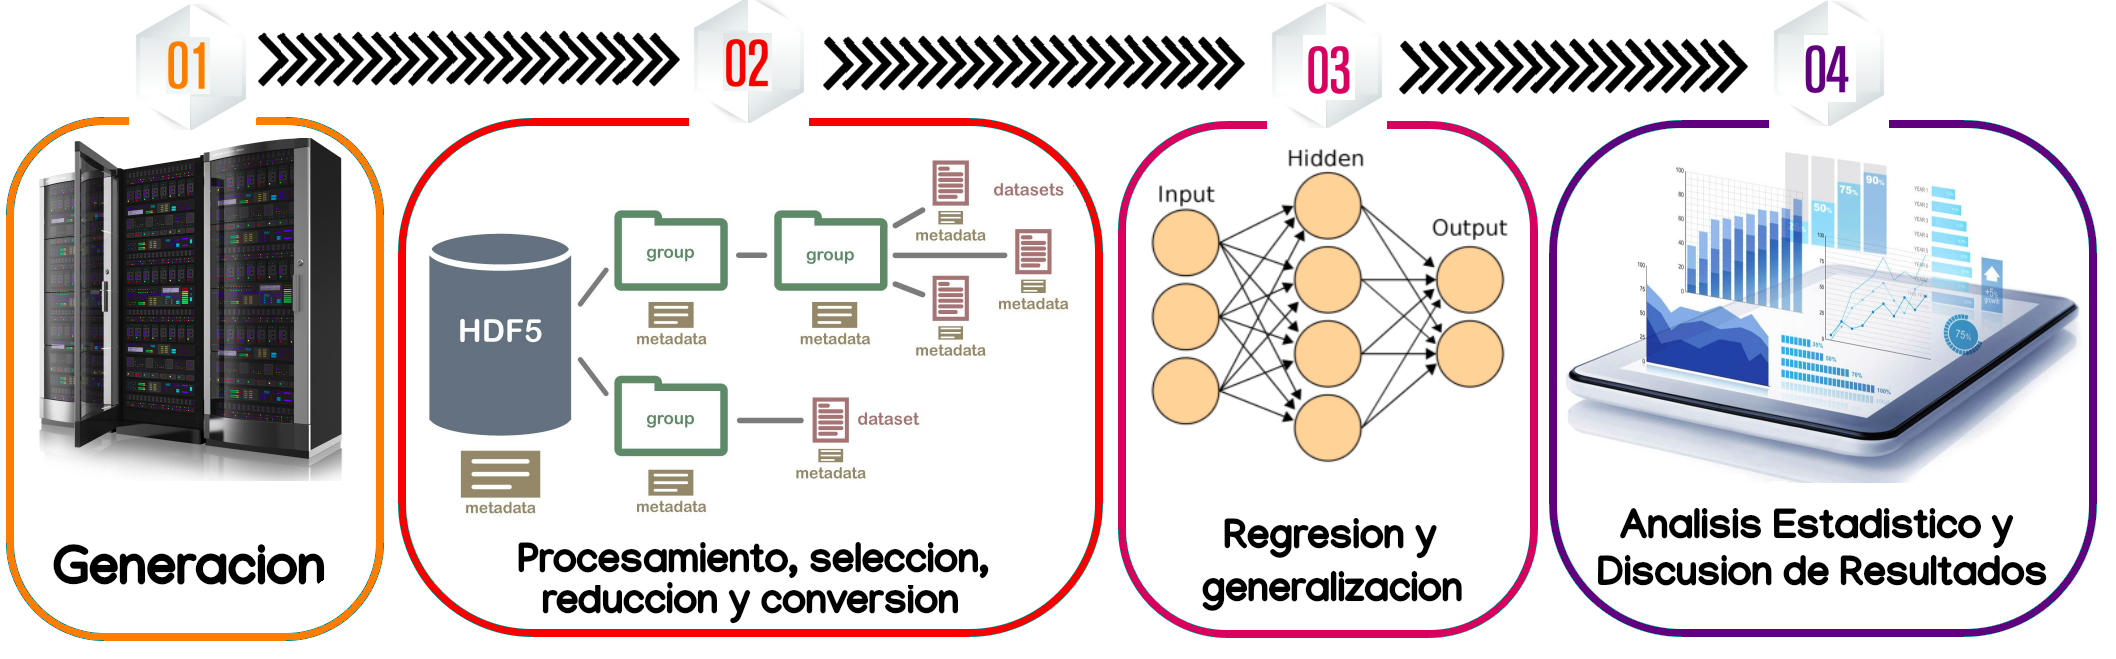
\includegraphics[width=1\textwidth]{Imag/procesos_darksusy.png}
\caption{Secuencia lógica de la investigación.}
\end{figure}

\framebreak

\begin{figure}[h]
\centering
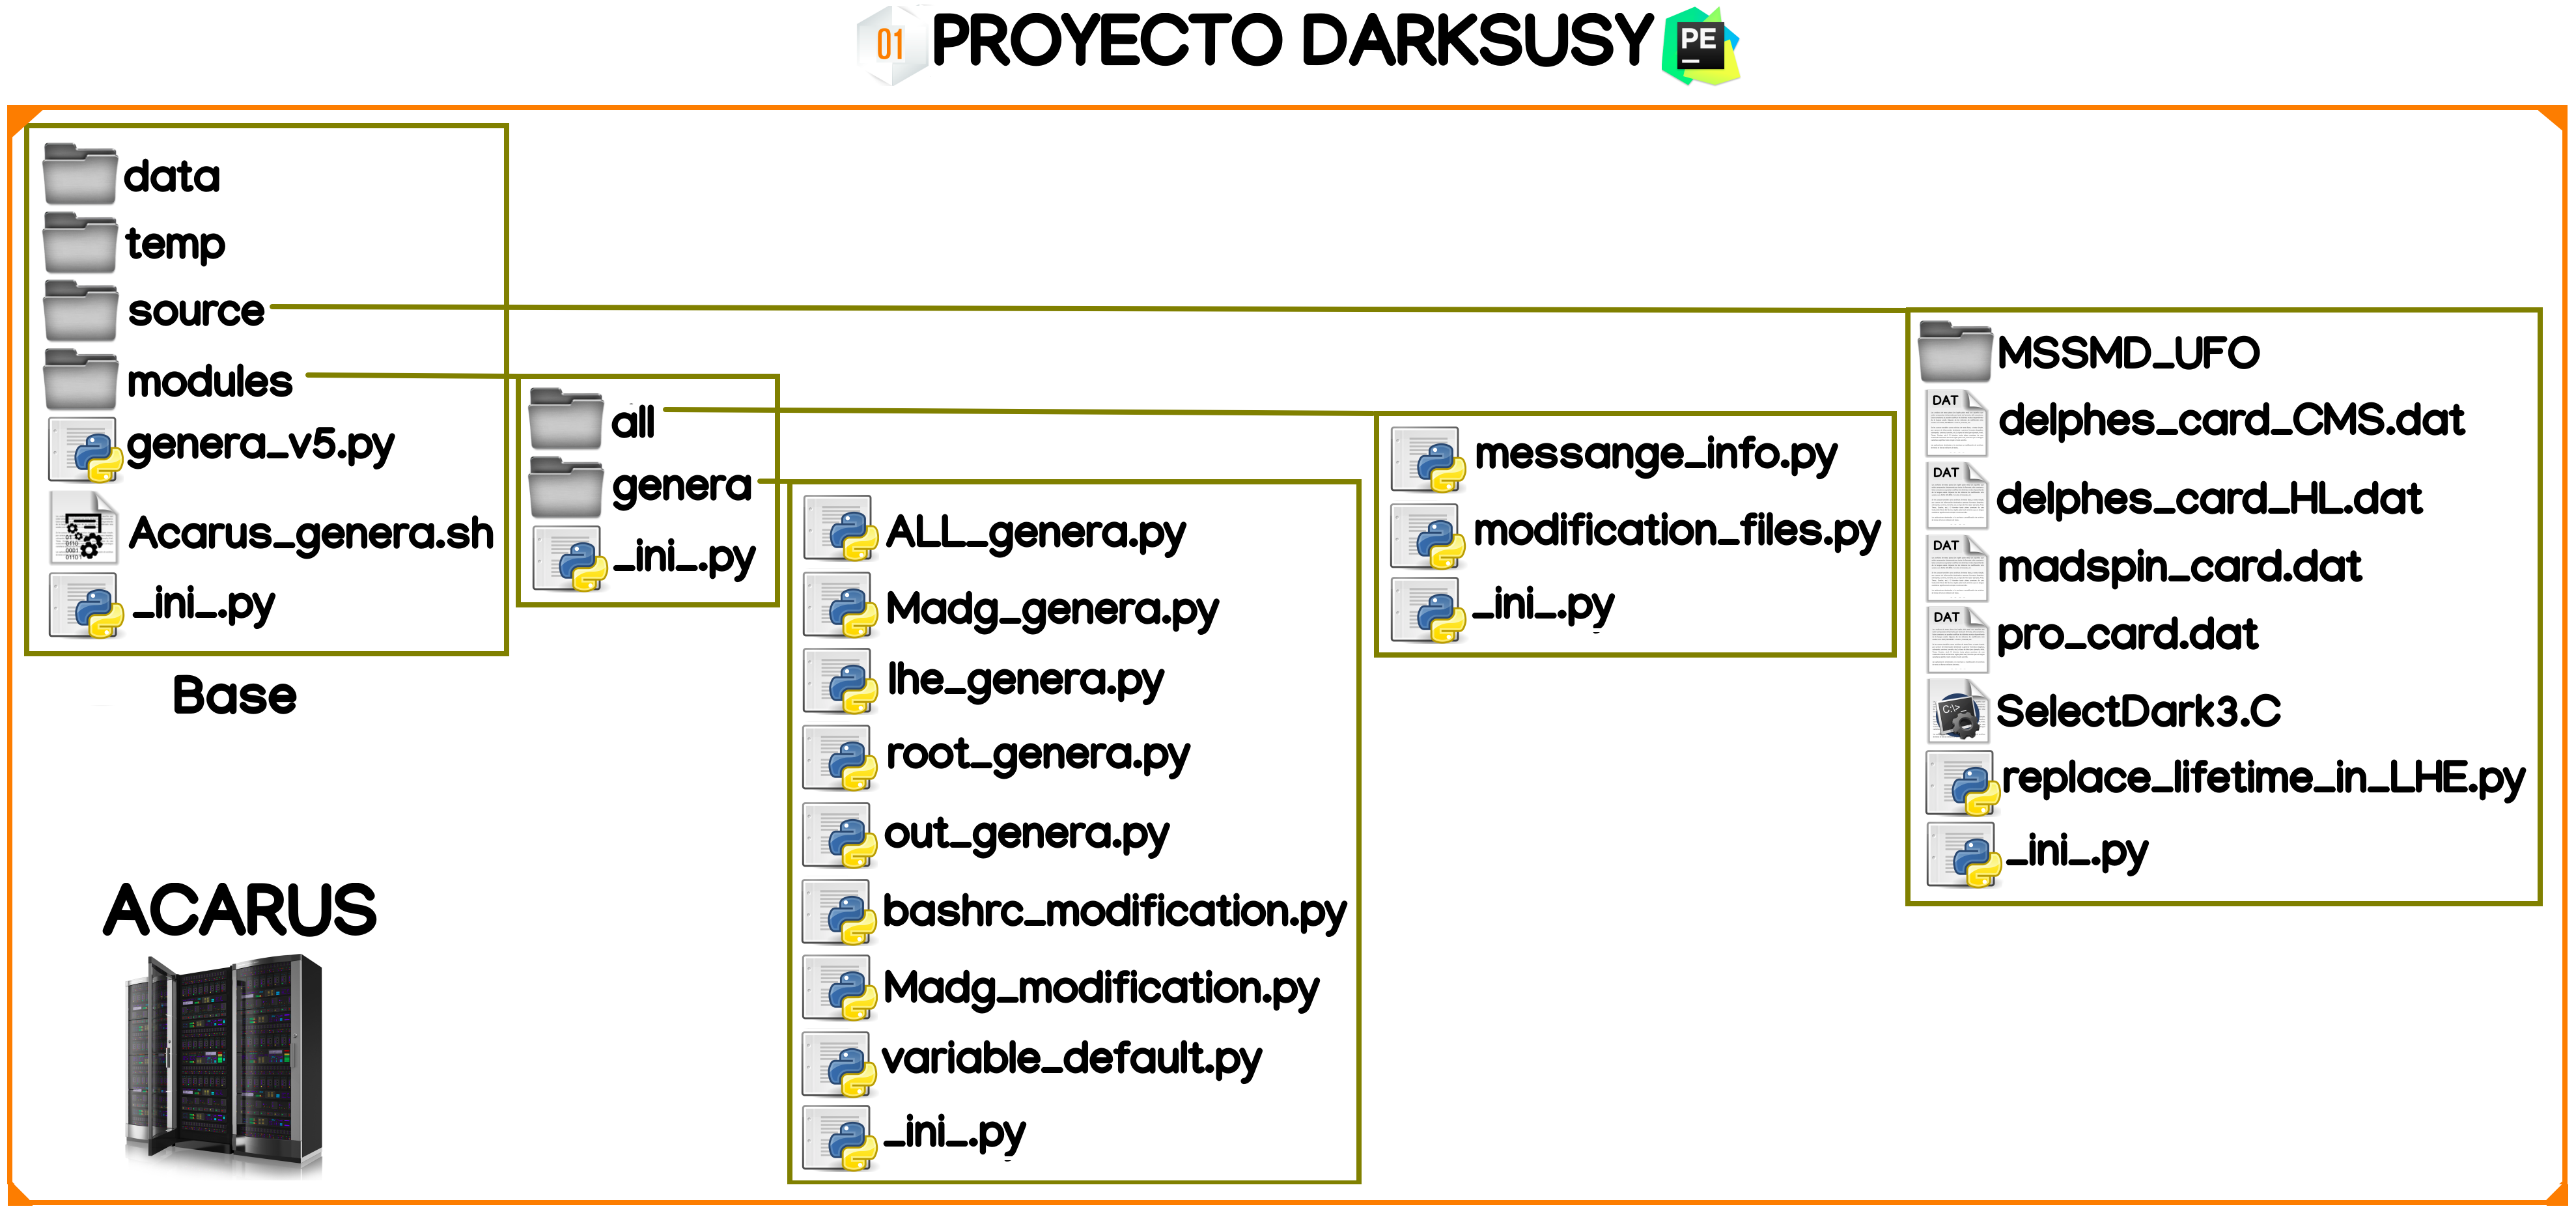
\includegraphics[width=1\textwidth]{Imag/proyecto_darksusy.png}
\caption{Estructura del proyecto generador.}
\end{figure}

\framebreak

\begin{figure}[h]
\centering
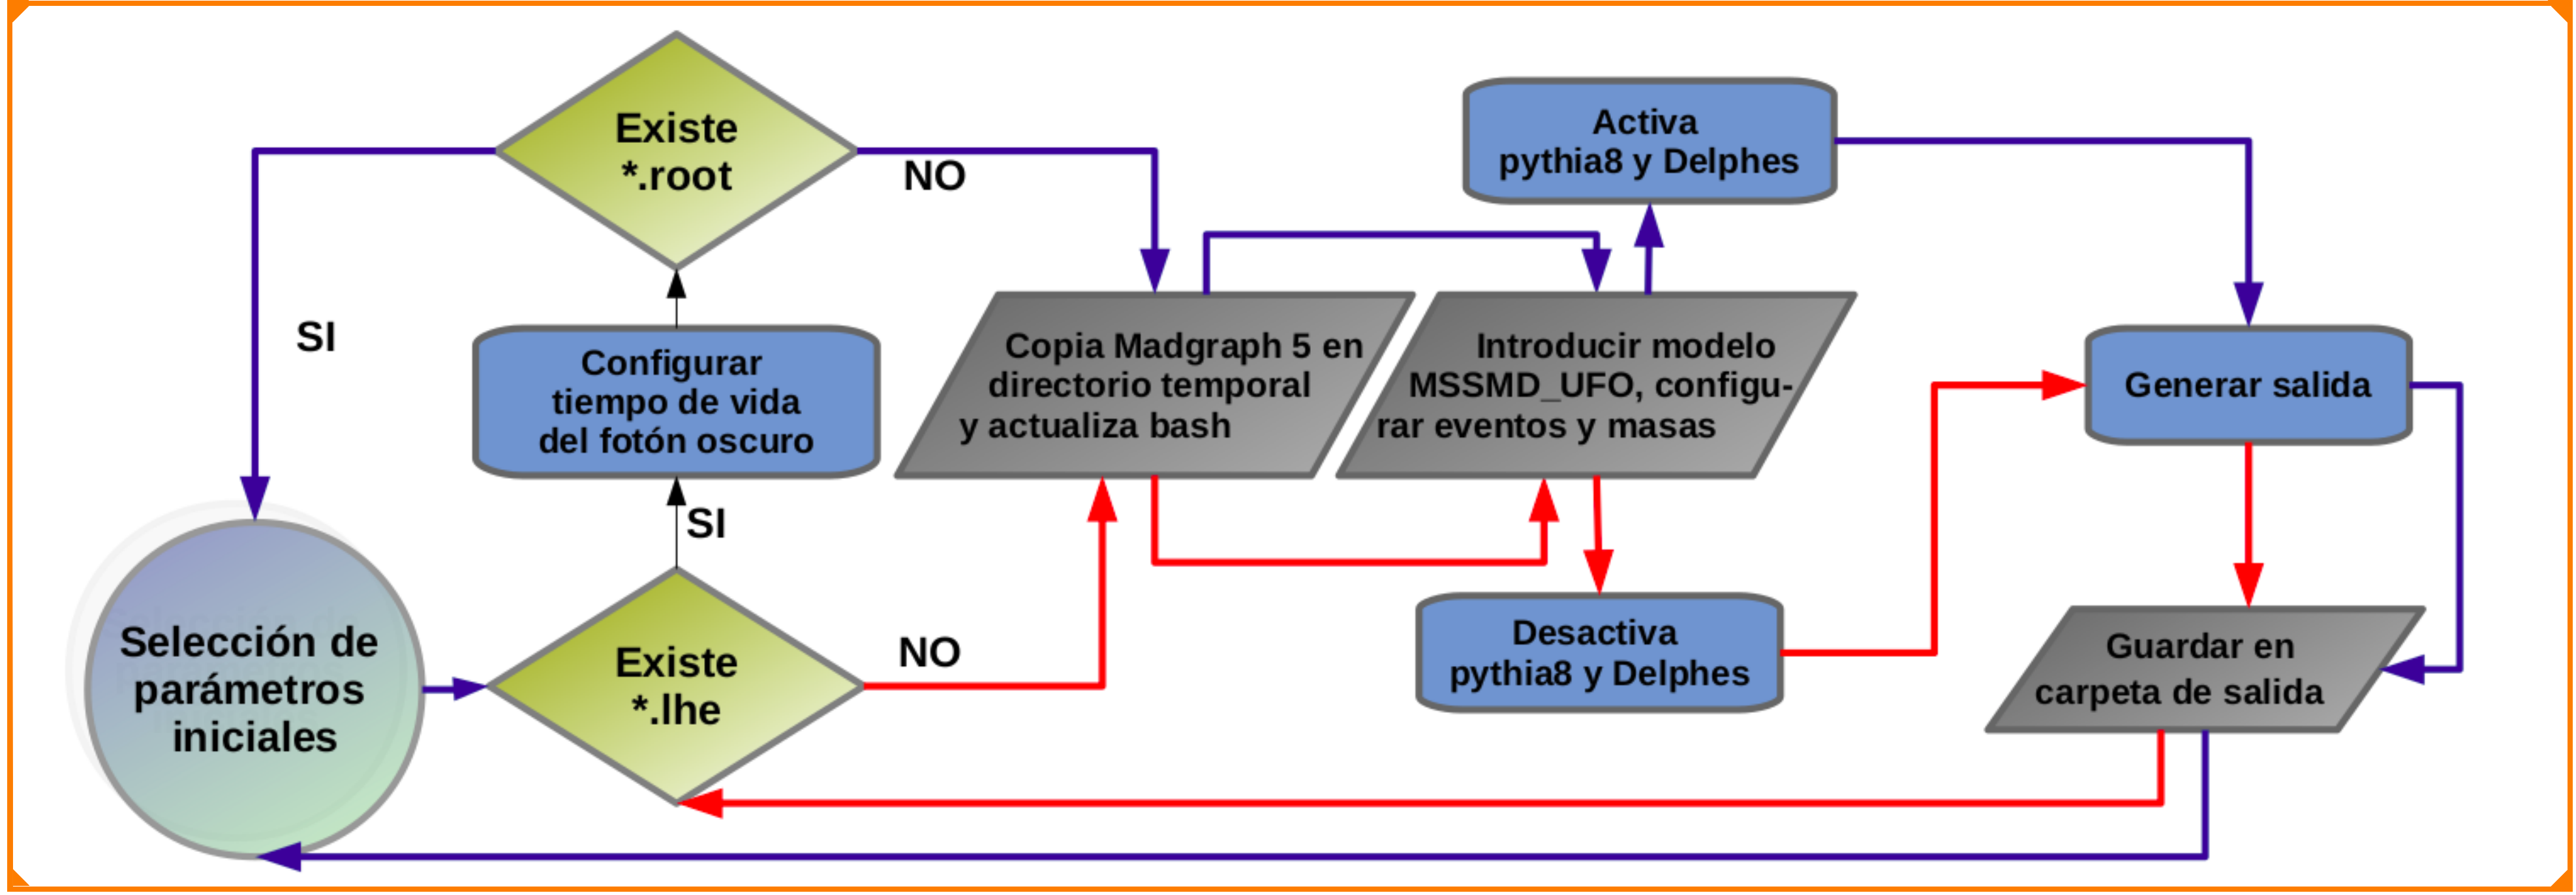
\includegraphics[width=1\textwidth]{Imag/proyecto_darksusy2.png}
\caption{Diagrama de Flujo del generador.}
\end{figure}

\framebreak

\begin{figure}[h]
\centering
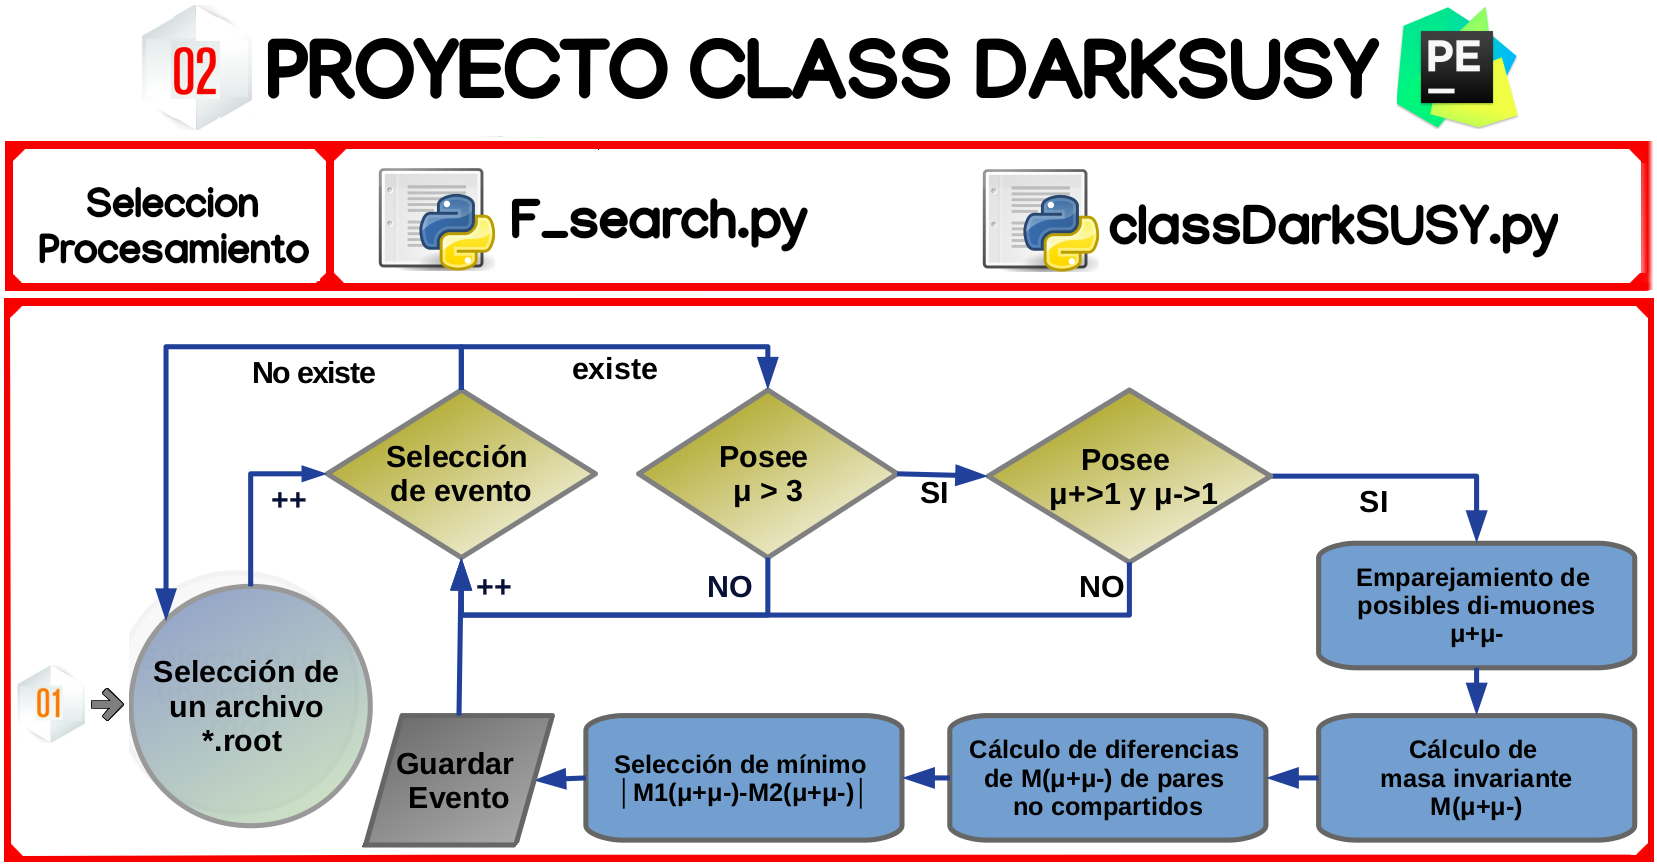
\includegraphics[width=1\textwidth]{Imag/class_darksusy.png}
\caption{Estructura del proyecto interpretador de la información $*.root$.}
\end{figure}

\framebreak

\begin{figure}[h]
\centering
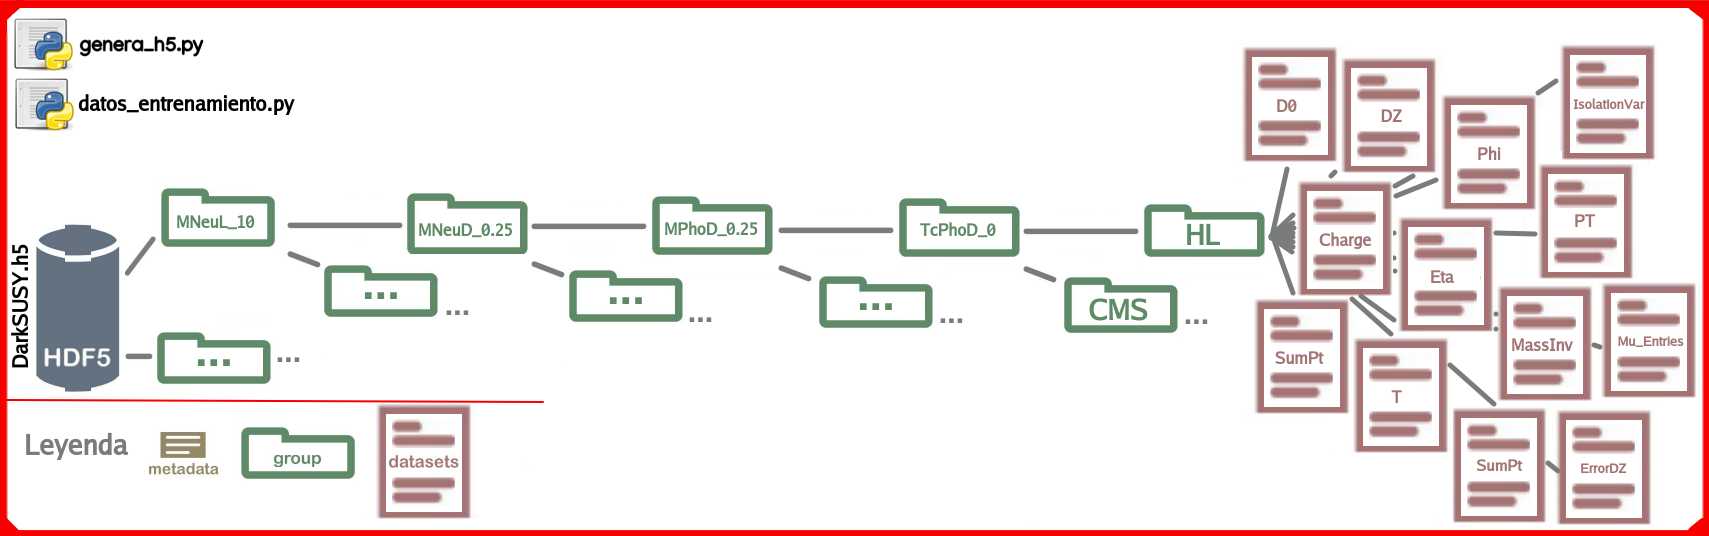
\includegraphics[width=1\textwidth]{Imag/class_darksusy3.png}
\caption{Estructura del archivo h5.}
\end{figure}
\end{frame}



\begin{frame}[fragile,allowframebreaks]{Análisis Preliminar. Análisis del contenido muónico}
\begin{figure}[h]
\centering
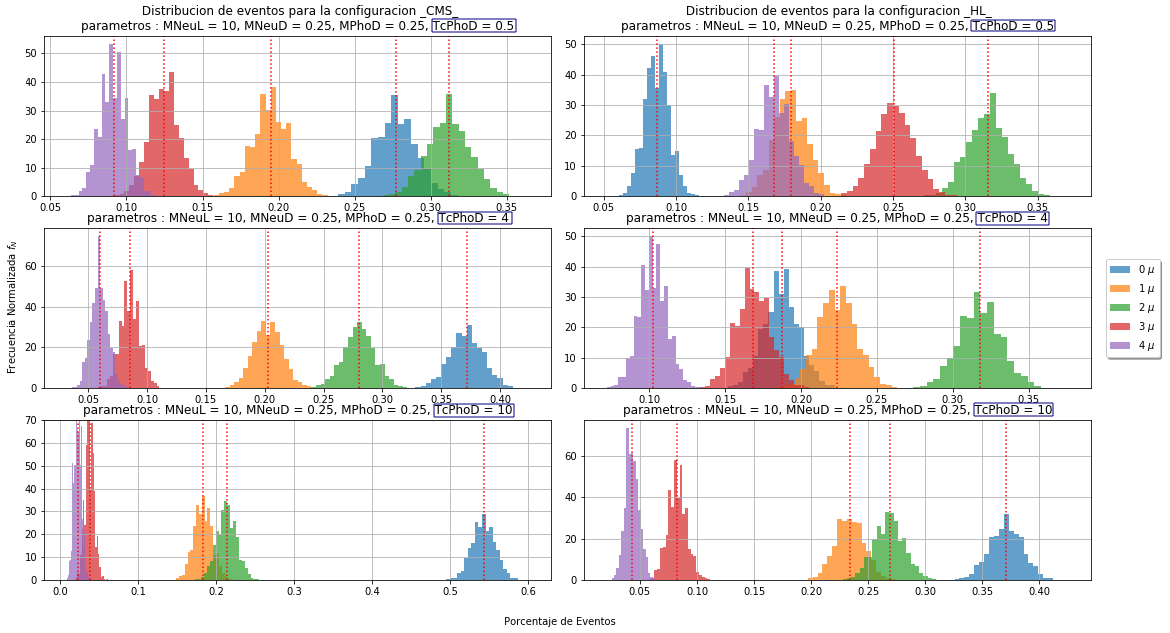
\includegraphics[width=.9\textwidth]{Imag/Distribucion_Entries.png}
\caption{Distribuciones de frecuencia de las entradas $f^{(j,~k)}$ ante cambios de \texttt{TcPhoD}.}
\end{figure}

\framebreak

\begin{figure}[h]
\centering
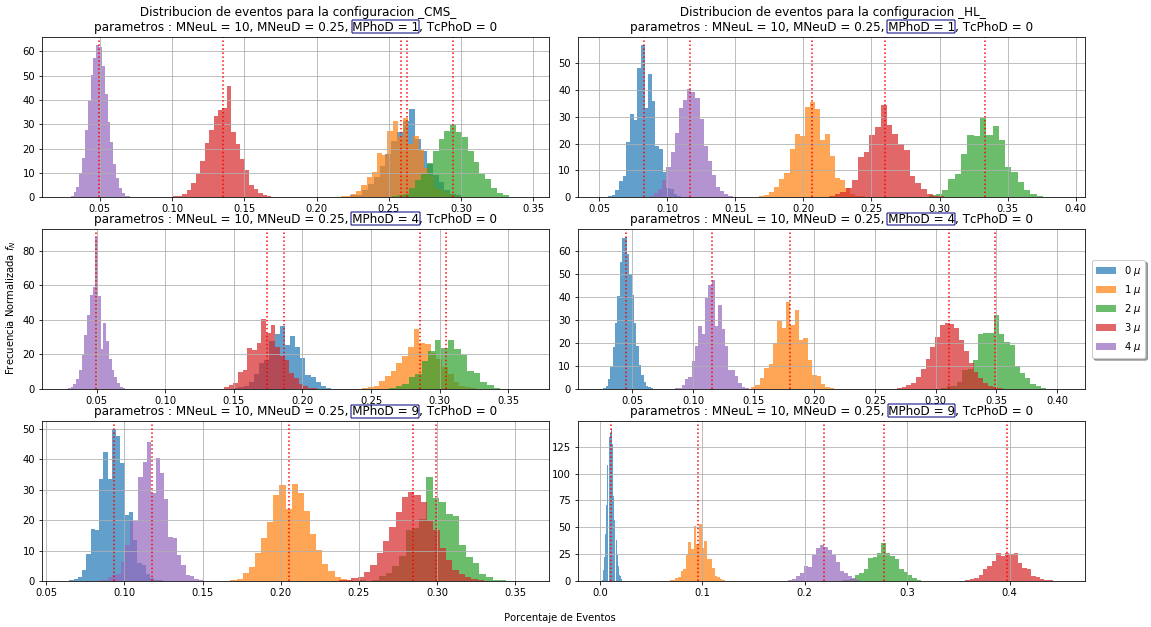
\includegraphics[width=.9\textwidth]{Imag/Distribucion_Entries2.png}
\caption{Distribuciones de frecuencia de las entradas $f^{(j,~k)}$ ante cambios de \texttt{MPhoD}.}
\end{figure}

\framebreak

\begin{figure}[h]
\centering
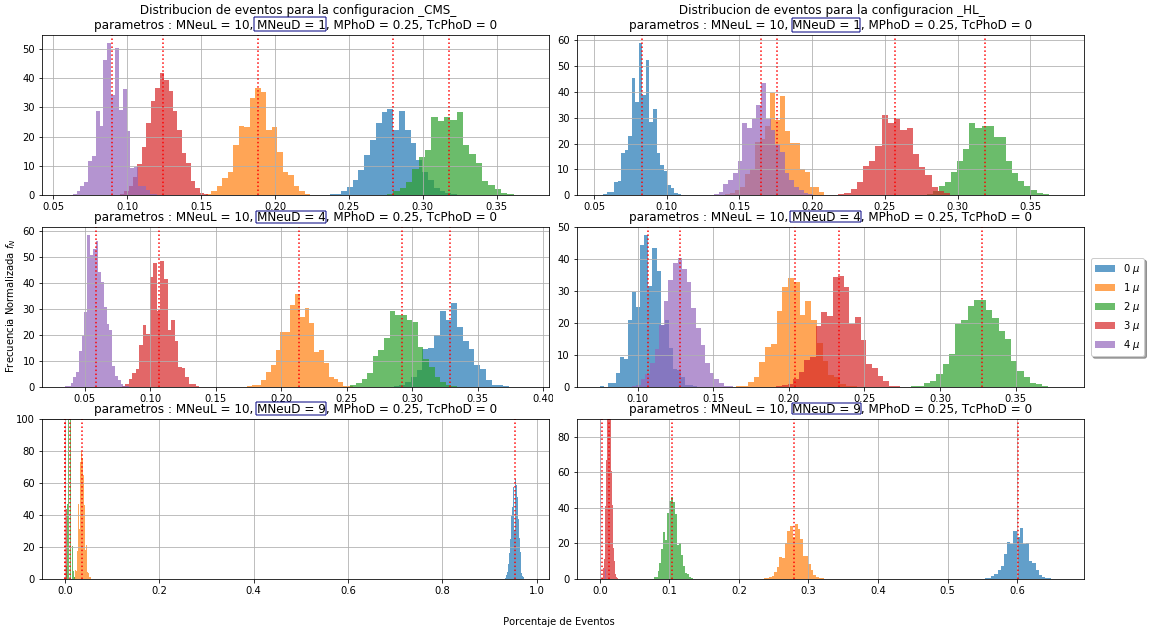
\includegraphics[width=.9\textwidth]{Imag/Distribucion_Entries3.png}
\caption{Distribuciones de frecuencia de las entradas $f^{(j,~k)}$ ante cambios de \texttt{MNeuD}.}
\end{figure}





\end{frame}